%preamble
\documentclass[12pt,a4paper]{article}

% for subfigure 
\usepackage{caption}
\usepackage{subcaption}
% to have reference and index in table of content
\usepackage{tocbibind}
% to have index
\usepackage{makeidx}
\makeindex

\usepackage{graphicx}
%\graphicspath{{figures/}}
\usepackage{amsmath}

\usepackage{hyperref}

% for tabels
\usepackage{multirow}
\usepackage[table,xcdraw]{xcolor}
% for khafan enumrate
\usepackage[inline]{enumitem}
%%%%%%%%%%%%%%%%%%%%%%%%%%
% xepersian and fonts
\usepackage{xepersian}
\settextfont{XBZar}
\setdigitfont{XBZar}
%%%%%%%%%%%%%
\defpersianfont\titr[Scale=1]{XB Zar}
\defpersianfont\nastaliq[Scale=1.5]{IranNastaliq}
\defpersianfont\traffic[Scale=1]{XM Traffic}
%%%%%%%%%%%%%%%%%%%%%%%%%%

%body
\begin{document}
	% to make page number letter instead of number
	\pagenumbering{harfi}
	% to remove page number in this page
	\thispagestyle{empty}
	\vspace*{-45mm}
	\centerline{
\includegraphics[height=4cm]{figures/srulogofa.png}}
	\begin{center}
		
		\vspace{-3mm}
		دانشکده مهندسی کامپیوتر
		\\[.2cm]
		
		گروه هوش مصنوعی و رباتیکز
		\\[0.7cm]
		{\Large 
			\textbf{گزارش پیشرفت سه ماهه پایان‌نامه کارشناسی‌ارشد}
			\\[0.2cm]
			از تاریخ ۱۳۹۹/۰۷/۰۱ تا ۱۳۹۹/۰۹/۳۰
		}
		\\[.2cm]
		\baselineskip=1.5cm
		{\titr
			\begin{huge}
				رابطه بين فعاليت‌های مغزی و مشخصه‌های چندرسانه‌ای آموزشي
			\end{huge}
		}
		\\[0.7cm]
		{\large
			{\traffic 
				اساتید راهنما
			}
			\\
			{\large \nastaliq دکتر رضا ابراهیم‌پور
			\\
		دکتر سید حمید امیری }
			\\[.7cm]
			{\traffic
				استاد مشاور
				\\
			}
			{\large \nastaliq دکتر علی‌رضا بساق‌زاده
			}
			\\[.5cm]
			{\large\traffic  پژوهشگر
			}
		}
		\\
		{\large \nastaliq امیرحسین اسعدی}
		\\
		پاییز ۱۳۹۹
	\end{center}
% to go to new page
\newpage
% to change distance between lines
\baselineskip=1cm
% to create table
\tableofcontents

%\newpage
%\listoftables

\newpage
\listoffigures

\newpage
\baselineskip=.75cm
% to change pagenumbers in persian digit
\pagenumbering{arabic}


% 1- Proposal Reveiw
\section{مقدمه}
\label{s:introduction}
امروزه با توسعه فناوری اطلاعات و ابزارهای نوین یادگیری و کاهش سهم آموزش رسمی در میان دانش‌آموزان و دانشجویان اهمیت نقش یادگیرنده و ابزارهای یادگیری مشخص می‌شود.
یکی از ابزار‌های نوین چندرسانه‌ای و فیلم‌های آموزشی است.کاهش فشار ذهنی یادگیرنده جزء اولویت‌های اصلی طراح چندرسانه‌ای آموزشی است.
فشار ذهنی می‌تواند از خود موضوع، رسانه انتقال و یا حاصل پردازش های شناختی یادگیرنده باشد.
\\
سنجش میزان بارشناختی ایجاد شده در یادگیرنده این امکان را می‌دهد تا بتوانیم با چیدمان و طراحی مناسب چندرسانه‌ای، کاهش بارشناختی یادگیرنده را مدیریت کنیم.
با ابزارهای مختلفی میتوان بارشناختی را سنجید که هریک مزایا و معایب خاص خود را دارد. در این پژوهش سعی شده است به طور خاص سنجش بار شناختی به وسیله داده‌هایی مختلفی که از چشم کاربر گرفته می‌شود مورد بررسی و مرور قرار گیرد.
\\
ساختار گزارش پیش‌رو با این شرح است در بخش
\ref{s:multimedia}
به اصول طراحی چندرسانه‌ای پرداخته می‌شود، این اصول با آزمایش های تجربی نشان داده شده‌ است که سبب کاهش میزان بارشناختی می‌شود. در بخش 
\ref{s:CognitiveLoad}
مفهوم بارشناختی و حافظه فعال ارائه می‌شود و سپس روش های متداول اندازه‌گیری بارشناختی معرفی خواهد شد.
در بخش 
\ref{s:eye}
به طور ویژه به سنجش بارشناختی به‌وسیله داده‌های چشمی و مغزی پرداخته می‌شود.
و در بخش 
\ref{s:data}
به نحوه پردازش داده‌ها و همچنین موارد مطالعه هریک پژوهش های مرتبط با داده‌های چشمی و مغزی در سنجش بار شناختی بررسی خواهد شد.
در نهایت در بخش
\ref{s:conclusion}
به نتیجه‌گیری و جمع‌بندی آن‌چه در این پژوهش مورد مطالعه قرار گرفته خواهیم پرداخت.
	
% 2- three month report
\section{گزارش پیشرفت دوره سه‌ماهه}
\subsection{فهرست فعالیت‌های انجام شده در این دوره (سه ماهه اول)}
\begin{enumerate}
	\item مطالعه‌ و پیاده‌سازی روش‌های پیش پردازش و استخراج ویژگی از سیگنال‌های مغزی
	\item مطالعه روش‌های تحلیل محتوای معنایی و زبانی
	\item  مطالعه روش‌های بررسی ارتباط میان سیگنال‌های مغزی و محتوای معنایی یک چندرسانه‌ای آموزش زبان  
\end{enumerate}
\subsection{شرح فعالیت‌ها و دستاورد‌های هر فعالیت در این دوره}
در این بخش شرح فعالیت‌ها و پیشرفت‌های انجام شده از آغاز پروژه تا تنظیم گزارش جاری بیان می‌شود. 
\begin{enumerate}
	\item
	{
		\begin{description}
			\item[عنوان فعالیت] مطالعه‌ و پیاده‌سازی روش‌های پیش پردازش و استخراج ویژگی از سیگنال‌های مغزی
			\item[دستاورد حاصل] داده‌های اخذ شده
			\cite{latifzadeh2020evaluating}
			با روش‌های جدیدتری از نویز‌های رایج سیگنال مغزی پاک سازی شدند. و ویژگی‌های متفاوتی نیز از آن‌ها استخراج شد.
			\item[ریز فعالیت‌ها]
			{
				\begin{enumerate*}
					\item یادگیری کار با نرم‌افزار EEGLAB که به منظور کار با سیگنال‌های مغزی طراحی شده است.
					\item یادگیری با افزونه‌های EEGLAB برای حذف نویز‌های متداول چون برق شهری، حرکت عضلات و پلک زدن طراحی شده‌اند.
					\item مطالعه روش‌های رایج و جدید برای استخراج ویژگی از سیگنال‌های مغزی.	
				\end{enumerate*}
			}
			\item[درصد پیشرفت (از ۱۰۰٪)] ۱۰۰	
			\item[توضحیات تکمیلی] در ادامه این گزارش آمده است.
	\end{description}
	}
	\item
	{
		\begin{description}
			\item[عنوان فعالیت] مطالعه روش‌های تحلیل محتوای معنایی و زبانی
			\item[دستاورد حاصل] دو روش متفاوت برای ارزیابی محتوای معنایی و زبانی چندرسانه‌ای بررسی، پیاده سازی و درنهایت ارزیابی شد.	
			\item[ریز فعالیت‌ها]
			{
				\begin{enumerate*}
					\item بررسی میزان پیچیدگی یک متن به لحاظ معنایی 
					\item میزان پیچیدگی یک متن به لحاظ ساختاری
					\item میزان فراوانی یک لغت در طول زمان
					\item ارزیابی روش‌های بیان شده
				\end{enumerate*}
			}
			\item[درصد پیشرفت (از ۱۰۰٪)] ۷۵ درصد	
			\item[توضحیات تکمیلی] در ادامه این گزارش آمده است.
		\end{description}
	}
	\item
	{
		\begin{description}
			\item[عنوان فعالیت] مطالعه روش‌های بررسی ارتباط میان سیگنال‌های مغزی و محتوای معنایی یک چندرسانه‌ای آموزش زبان\\
			
			\item[دستاورد حاصل] مشخص شدن مکان‌ها و زمانن‌هایی از مغز که بیشترین وابستگی را به معیار‌های زبانی دارند	
			\item[ریز فعالیت‌ها]
			{
				\begin{enumerate*}
					\item بررسی معیار‌های وابستگی میان دو سیگنال
					\item مطالعه پژوهش‌های مربوطه در این زمینه	
				\end{enumerate*}
			}
			\item[درصد پیشرفت (از ۱۰۰٪)] ۵۰ درصد	
			\item[توضحیات تکمیلی] در ادامه این گزارش آمده است.
		\end{description}
	}

\end{enumerate}
\subsection{گزارش تکمیلی فعالیت‌ها}
\subsubsection{پردازش سیگنال‌های مغزی}
در این قسمت سیگنال های خام اخذ شده 
\cite{latifzadeh2020evaluating}
با نرم افزار EEGLAB
\cite{delorme2004eeglab}
که یکی از بسته‌های متن باز متلب است پیش پردازش شدند. در ابتدا فرکانس‌های ۴۰ تا ۵۰ هرتز که مربوط به نویز برق شهری هستند حذف شدند. بعد از آن به کمک افزونه ASR برخی از اعمال چون: حذف بازه‌ای از سیگنال که در آن به مدت ۵ ثانیه ثابت باشد، فرکانس‌های زیر یک هرتز،‌ حذف کانال‌هایی که با کانال‌های اطراف خود همبستگی کمی دارند و بازه‌هایی از سیگنال که در آن پرش شدیدی وجود دارد.
\newline
 سپس به کمک افزونه‌ای که مولفه‌های سیگنال مغزی را استخراج می‌کند مولفه‌های غیر مغزی حذف شدند. این مولفه‌ها شامل پلک زدن، حرکت چشم‌ها، فرو بردن آب دهان، حرکت سر، نفس کشیدن و حرکت دندان‌ها هستند.
\subsubsection{تحلیل محتوای‌ معنایی و زبانی}
در این بخش متن گفتار چندرسانه‌ای آماده شده که زمان آن
$3'\text{:}41''$
و شامل ۷۸۲ کلمه بود با معیارهای متفاوتی مورد ارزیابی قرار گرفت. هدف از انجام این کار سنجش میزان پیچیدگی گفتار و فعالیت که ممکن است در مغز ایجاد کند بود. این کار با دو دسته معبار متفاوت انجام شد. نخست معیار کوماتریس 
\cite{castro2020validating}
استفاده شد در این معیار متن از از دو جنبه سهولت خواندن و سادگی ساختار مورد بررسی قرار گرفت.
\newline
سهولت خواندن خود از پارامتر‌هایی چون طول جمله، تعداد کلمات و تعداد سیلابس ها تشکیل شده است. و خروجی آن عددی در بازه ۱ تا ۱۰۰ است که هرچه بزرگتر باشد متن ساده تر بوده و برعکس. سادگی ساختار نیز متن را به لحاظ تعداد ضمیرها فاصله تا اسم مورد نظر واین دست موارد بررسی می‌کند. و خروجی آن همانند سهولت خواندن است. 
\newline
معیار بعدی فراوانی لغت
\LTRfootnote{Word Frequency}
است
\cite{brodbeck2018neural}.
در این معیار یک مخزن عظیم لغات در نظر گرفته می‌شود سپس میزان رخداد هر کلمه مجزا در آن محاسبه شده و اعلام می‌شود. به عنوان نمونه می‌توان تمام زیرنویس فیلم‌های موجود را یک مخزن عظیم داده در نظر گرفت و یا متن روزنامه‌های آنلاین. 
یک مسئله در این روش پیدا کردن زمان شروع و پایان گفتار یک کلمه است. برای این منظور ابتدا از شبکه عصبی که به این منظور آموزش دیده به نام Gentle استفاده شد و سپس برای دقیق شدن خروجی آن زمان‌های شروع و اتمام تمامی کلمات به صورت دستی با نرم‌افزار Praat تمیز شد. مزیت این روش نسبت به روش قبلی داشتن دقت زمانی بالا است.
\subsubsection{ارتباط میان سیگنال‌های مغزی و محتوای معنایی}
در این بخش معیار های متفاوت همبستگی
\LTRfootnote{Correlation}
مطالعه و مورد بررسی قرار گرفت. این معیار همبستگی شباهت میان دو مجموعه داده را می‌سنجد و خروجی آن عددی بین صفر تا یک است. هر چه این عدد به سمت صفر نزدیک‌تر باشد دو مشاهده مورد نظر همبستگی کمتری دارند و هرچه به سمت یک و منفی یک باشد همبستگی بیشتری دارند.
\newline
نوع دیگر از آن هبستگی کانونی
\LTRfootnote{Canonical Correlation}
است، که در آن همبستگی خطی میان چند مشاهده و چند مشاهده دیگر اندازه گیری می‌شود. می‌توان گفت این روش از این جهت که تمامی مشاهدات در نظر گرفته می‌شود و از هر کدام ضریبی در نظر گرفته شده دقیق‌تر است.
حال می‌توان ضریب‌ها در توپوگرافی مغز رسم نمود و نواحی مرتبط با پردازش کلمات در مغز را شناسایی نمود و یا با جابه‌جا کردن سیگنال در زمان با واحدهای کوچک مثلا پنجاه میلی ثانیه بررسی نمود که مغز در چه زمانی پس از نشان دادن محرک به آن پاسخ می‌دهد.
شکل 
کارهای انجام شده را نشان می‌دهد.
\begin{figure}[h]
	\centering
	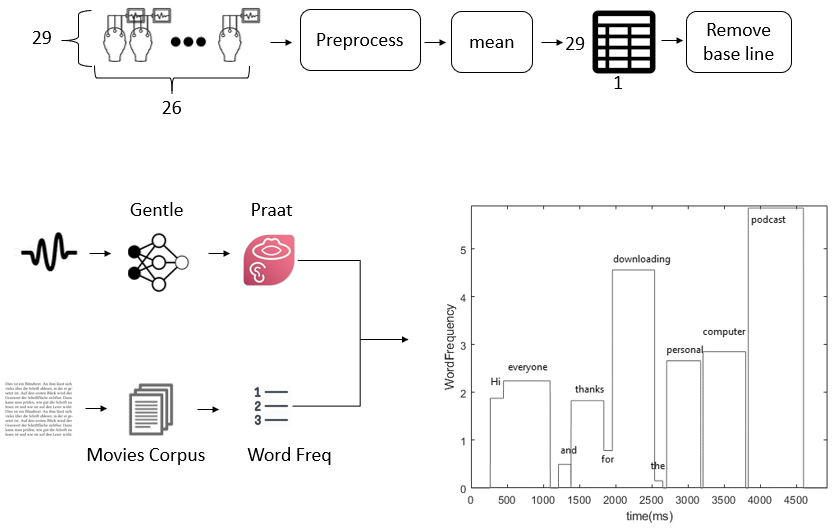
\includegraphics[width=0.8\linewidth]{figures/procedure}
	\caption[رویه‌ کار‌های انجام شده]{سیگنال‌های مغزی پس از پیش پردازش میانگین گرفته شده و ثانیه‌های ابتدایی آن که مربوط به حالت استراحت کاربر است حذف می‌شوند. از سوی دیگر گفتار و کلمات آن تحلیل می‌شوند و سیگنالی از فراوانی هر لغت در زمان آماده می‌شوند }
	\label{fig:procedure}
\end{figure}

\subsection{برنامه و زمان‌بندی ادامه اجرای پروژه}
انتظار می‌رود در سه ماهه دوم این اهداف و فعالیت‌ها محقق شوند:
\begin{enumerate}
	\item اتمام و جمع‌بندی رابطه میان گفتار چندرسانه‌ای به لحاظ زبانی و معنایی با فعالیت‌های مغزی
	\item بررسی جنبه‌های دیگر محتوای چندرسانه‌ای آموزشی همچون فیلم و فعالیت‌های مغزی
\end{enumerate}
%make it left to right
\setLTRbibitems
\bibliographystyle{ieeetr-fa}
\bibliography{references_BIBTEX}

\end{document}